\documentclass[conference]{IEEEtran}
\IEEEoverridecommandlockouts
% The preceding line is only needed to identify funding in the first footnote. If that is unneeded, please comment it out.
\usepackage[english]{babel}
\usepackage{amsthm}
\usepackage{cite}
\usepackage{amssymb,amsfonts}
\usepackage{algorithmic}
\usepackage{graphicx}
\usepackage{textcomp}
\usepackage{xcolor}
\usepackage[fleqn]{amsmath}
\usepackage[a4paper, total={184mm,239mm}]{geometry}
\def\BibTeX{{\rm B\kern-.05em{\sc i\kern-.025em b}\kern-.08em
    T\kern-.1667em\lower.7ex\hbox{E}\kern-.125emX}}

\theoremstyle{definition}
\newtheorem{definition}{Definition}
\usepackage{listings}
\usepackage{stfloats}
\usepackage{graphicx}
\usepackage{caption}
\usepackage{xcolor}
% \usepackage[fleqn]{amsmath}
\usepackage{lstautogobble}  % Fix relative indenting
\usepackage{color}          % Code coloring
\usepackage{zi4}            % Nice font

\definecolor{bluekeywords}{rgb}{0.13, 0.13, 1}
\definecolor{graycomments}{rgb}{0.5, 0.5, 0.5}
\definecolor{redstrings}{rgb}{0.9, 0, 0}
\definecolor{graynumbers}{rgb}{0.5, 0.5, 0.5}

\lstset{
    autogobble,
    columns=fullflexible,
    showspaces=false,
    showtabs=false,
    breaklines=true,
    showstringspaces=false,
    breakatwhitespace=true,
    escapeinside={(*@}{@*)},
    commentstyle=\color{graycomments},
    keywordstyle=\color{bluekeywords},
    stringstyle=\color{redstrings},
    numberstyle=\color{graynumbers},
    basicstyle=\ttfamily,
    xleftmargin=18pt,
    xrightmargin=2pt,
    tabsize=4,
    captionpos=b
}
\lstset
{ %Formatting for code in appendix
    language=Matlab,
    % basicstyle=\footnotesize,
    numbers=left,
    stepnumber=1,
    showstringspaces=false,
    tabsize=1,
    breaklines=true,
    breakatwhitespace=false,
}
\lstset{
numbers=left, 
numberstyle=\small, 
numbersep=8pt, 
frame = single, 
language=Pascal, 
framexleftmargin=15pt}

\pagestyle{empty}
\begin{document}

\title{RVFC: RISC-V Formal in Chisel
% {\footnotesize \textsuperscript{*}Note: Sub-titles are not captured in Xplore and
% should not be used}
% \thanks{Identify applicable funding agency here. If none, delete this.}
}

% \author{\IEEEauthorblockN{1\textsuperscript{st} Given Name Surname}
% \IEEEauthorblockA{\textit{dept. name of organization (of Aff.)} \\
% \textit{name of organization (of Aff.)}\\
% City, Country \\
% email address or ORCID}
% \and
% \IEEEauthorblockN{2\textsuperscript{nd} Given Name Surname}
% \IEEEauthorblockA{\textit{dept. name of organization (of Aff.)} \\
% \textit{name of organization (of Aff.)}\\
% City, Country \\
% email address or ORCID}
% \and
% \IEEEauthorblockN{3\textsuperscript{rd} Given Name Surname}
% \IEEEauthorblockA{\textit{dept. name of organization (of Aff.)} \\
% \textit{name of organization (of Aff.)}\\
% City, Country \\
% email address or ORCID}
% \and
% \IEEEauthorblockN{4\textsuperscript{th} Given Name Surname}
% \IEEEauthorblockA{\textit{dept. name of organization (of Aff.)} \\
% \textit{name of organization (of Aff.)}\\
% City, Country \\
% email address or ORCID}
% \and
% \IEEEauthorblockN{5\textsuperscript{th} Given Name Surname}
% \IEEEauthorblockA{\textit{dept. name of organization (of Aff.)} \\
% \textit{name of organization (of Aff.)}\\
% City, Country \\
% email address or ORCID}
% \and
% \IEEEauthorblockN{6\textsuperscript{th} Given Name Surname}
% \IEEEauthorblockA{\textit{dept. name of organization (of Aff.)} \\
% \textit{name of organization (of Aff.)}\\
% City, Country \\
% email address or ORCID}
% }

\maketitle

\begin{abstract}
    DUMMY ABSTRACT.
    Modern digital hardware is becoming ever more complex. And agile development, an efficient idea in software development, has been introduced into hardware. Furthermore, as a new hardware construction language, Chisel helps to raise the level of hardware design abstraction with the support of object-oriented and functional programming. Chisel plays a crucial role in future hardware design and open-source hardware development. However, the formal verification for Chisel is still limited. In this paper, we propose ChiselFV, a formal verification framework that has supported detailed formal hardware property descriptions and integrated mature formal hardware verification flows based on SymbiYosys. It builds on top of Chisel and uses Scala to drive the verification process. Thus the framework can be seen as an extension of Chisel. ChiselFV makes it easy to verify hardware designs formally when implementing them in Chisel.
\end{abstract}

\begin{IEEEkeywords}
RISC-V, Formal Verification, Hardware verification, Chisel
\end{IEEEkeywords}

\section{Introduction}
The dominant traditional hardware-description languages (HDLs), Verilog and VHDL, were originally developed as hardware simulation languages, and were only later adopted as a basis for hardware synthesis. 
These languages also lack the powerful abstraction facilities that are common in modern software languages, which leads to low designer productivity by making it difficult to reuse components.
% 因此 Chisel 被推出。
Therefore, Chisel was proposed.
It is intended to be a simple platform that provides modern programming language features for accurately specifying low-level hardware blocks, but which can be readily extended to capture many useful high-level hardware design patterns \cite{bachrach2012chisel}.

% Chisel
Chisel (Constructing Hardware in a Scala-Embedded Language) is an open-source hardware construction language developed by UC Berkeley. It is developed as a domain-specific extension to the Scala programming language. And because Chisel is embedded in Scala, hardware developers can tap into Scala’s modern programming language features—such as object-oriented programming, functional programming, parameterized types, abstract data types, operator overloading, and type inference—to improve designer productivity by raising the abstraction level and increasing code reuse \cite{lee2016agile}.

% RISC-V
% Chisel 是为了敏捷开发 RISC-V 处理器而开发的,其生态因为其语言特性和 RISC-V 的流行而逐渐壮大。
Chisel was developed for agile development of RISC-V processors, and its ecosystem has grown due to its language features and the popularity of RISC-V.
RISC-V is an ISA developed at UC Berkeley and designed from the ground up to be clean, microarchitecture-agnostic and highly extensible. Most importantly, RISC-V is free and open, which allows it to be used in both commercial and open-source settings \cite{asanovic2014instruction}.
% UC Berkeley 也推出了两款具有代表性的基于 Chisel 的 RISC-V 芯片生成器。
UC Berkeley has also released two representative RISC-V chip generators based on Chisel: Rocket Chip \cite{asanovic2016rocket} and BOOM \cite{celio2017boomv2}.
% 这其中后者是一个乱序核。
The latter is an out-of-order core.
% Chisel 由于其高级语言的特性,提供了更强的抽象能力,从而提供了便利的库开发能力。
Chisel, due to its high-level language features, provides more powerful abstraction capabilities, thus providing convenient library development capabilities. 
% 前文中提到的 Rocket chip 实际上是一个 Chip 生成器,它由一系列的参数化的构建芯片库构成。
The Rocket Chip mentioned above is actually a chip generator, which consists of a collection of parameterized chip-building libraries that we can use to generate different SoC variants \cite{asanovic2016rocket}.
% 基于它的 Raven 系列芯片已经可以进行流片了。
The Raven family of chips based on it have already been taped out \cite{lee2015raven}.

% 验证的重要性,但是目前的处理器验证主要是在 SystemVerilog 层次。
% 在硬件开发流程中,由于其错误的代价十分高昂,设计的正确性验证是至关重要的。
In the hardware development process, due to the high cost of errors, the correctness verification of the design is crucial.
% 然而当前的处理器验证工作主要是在 SystemVerilog 层次。
However, current processor verification efforts are mainly at the SystemVerilog level.
% 对于 RISC-V 指令集处理器验证的代表性工作为 RISC-V Formal。
The representative work for RISC-V instruction set processor verification is RISC-V Formal \cite{riscv-formal}.
% RISC-V Formal 实现了什么,但是,不足:1. 层次 2. 框架结构
% RISC-V Formal 包含了一个处理器独立的 RISC-V ISA 形式化描述一组验证 testbench。
RISC-V Formal consists of a processor-independent formal description of the RISC-V ISA and a set of formal testbenches for each processor supported by the framework.
% 实现了 RISC-V Formal 中定义的 RVFI(RISC-V Formal Interface) 接口的 RISC-V core 都可以使用它进行形式化验证。
Any RISC-V core that implements the RVFI (RISC-V Formal Interface) defined in RISC-V Formal can use it for formal verification.
% 然而,RISC-V Formal 验证框架是在 SystemVerilog 层次的。
However, the RISC-V Formal verification framework is at the SystemVerilog level.
% 基于之前对于 Chisel 的说明和一些比较的工作,相比底层 HDL 语言,例如 SystemVerilog,Chisel 在设计和验证上都更具有生产力。
Based on the previous description of Chisel and some comparative work, Chisel is more productive in design and verification than low-level HDL languages, such as SystemVerilog \cite{im2021comparative}.
% 同时, Chisel 生成的 SystemVerilog 代码的可读性和可修改性较差,因此无法直接使用 RISC-V Formal 对 Chisel 实现的 Core 进行形式化验证。
At the same time, the readability and modifiability of the SystemVerilog code generated by Chisel is poor, it is not possible to directly use RISC-V Formal to verify the core implemented by Chisel.
% 另一方面,RISC-V Formal 的验证后端与框架是紧密耦合的,目前只支持调用 BMC 算法。
On the other hand, the verification backend of RISC-V Formal is tightly coupled with the framework, and currently only supports calling the BMC algorithm.

% 我们的贡献
% 基于上述,我们提出 RVFC 框架,受启发于 RISC-V Fomal 框架,并在 Chisel 层次进行实践。
Base on the above, we propose the RVFC (RISC-V Formal in Chisel) framework, inspired by the RISC-V Formal framework, and try to practice it at the Chisel level. 
% ChiselFV
% RVFC 框架基于我们之前的工作 ChiselFV。
The RVFC framework is based on our previous work ChiselFV \cite{ChiselFV}.
% ChiselFV 提供了在 Chisel 层次形式化定义性质,并可以进行一键式调用验证的能力。
ChiselFV provides the ability to formally define properties at the Chisel level and allows for one-click call verification.
% RVFC 相关的代码和 case 都可以在 GitHub 仓库中找到。
The related code and case of RVFC can be found in the GitHub repository \cite{riscvFvChisel}.
The main contributions of this work are as follows:

\begin{itemize}
    \item \textbf{RVFC framework.} 
    We propose the RVFC framework, which is a formal verification framework for RISC-V cores implemented in Chisel. The framework is inspired by the RISC-V Formal framework and is implemented at the Chisel level.
    % 借助 Chisel 中高级语言的特性,RVFC 框架实现了模块化和更好的扩展性。
    And the RVFC framework enables modularity and better extensibility thanks to the high-level language features in Chisel.
    % 验证流程
    \item \textbf{Verification flow.}
    % 我们使用 Chisel 按照教科书中使用 SystemVerilog 实现的一个五级流水案例进行了重新实现,并将其作为 Study case,实践 RVFC 验证框架下对 RISC-V 处理器的验证流程。
    We reimplemented a five-stage pipeline example using Chisel as described in the textbook \cite{patterson2017computer} using SystemVerilog and used it as a study case to practice the verification flow of RVFC verification framework for RISC-V processors.
\end{itemize}

% 文章组织
This paper is organized as follows. Section II introduces the RISC-V Formal framework. Section III details the design and workflow of the RVFC framework. 
% 一个在 Chisel 层次实现的五级流水设计和验证过程在 section IV 中以一个 study case 展示。
A five-stage pipeline design and verification process is presented in section IV as a study case.
Section V concludes.

\section{RISC-V Formal}

RISC-V Formal is a formal verification IP for RISC-V processors.
It is ongoing development and currently supports RV32/64IMC instruction set \cite{riscvf}.
RISC-V Formal consists of a processor-independent formal description of the RISC-V ISA and a set of formal testbenches for each processor supported by the framework.
% 该框架的验证对象在 Verilog/SystemVerilog 层次实现的 RISC-V 处理器,同时要求其实现了 RVFI 接口。
The framework verifies RISC-V processors implemented at the Verilog/SystemVerilog level and requires that they implement the RVFI interface.
% 它使用了 SVA(SystemVerilog Assertions) 在 SystemVerilog 上来定义形式化性质描述。
It uses SVA (SystemVerilog Assertions) \cite{vijayaraghavan2005practical} to define formal property descriptions on SystemVerilog.
% 验证后端则是将 SystemVerilog 和 SVA 代码直接交给 SymbiYosys 工具进行 BMC 检查。
The verification backend is a direct handoff of the SystemVerilog and SVA code to the SymbiYosys \cite{SymbiYosys} tool for BMC checking.

\begin{figure}[!htbp]
    \begin{center}
    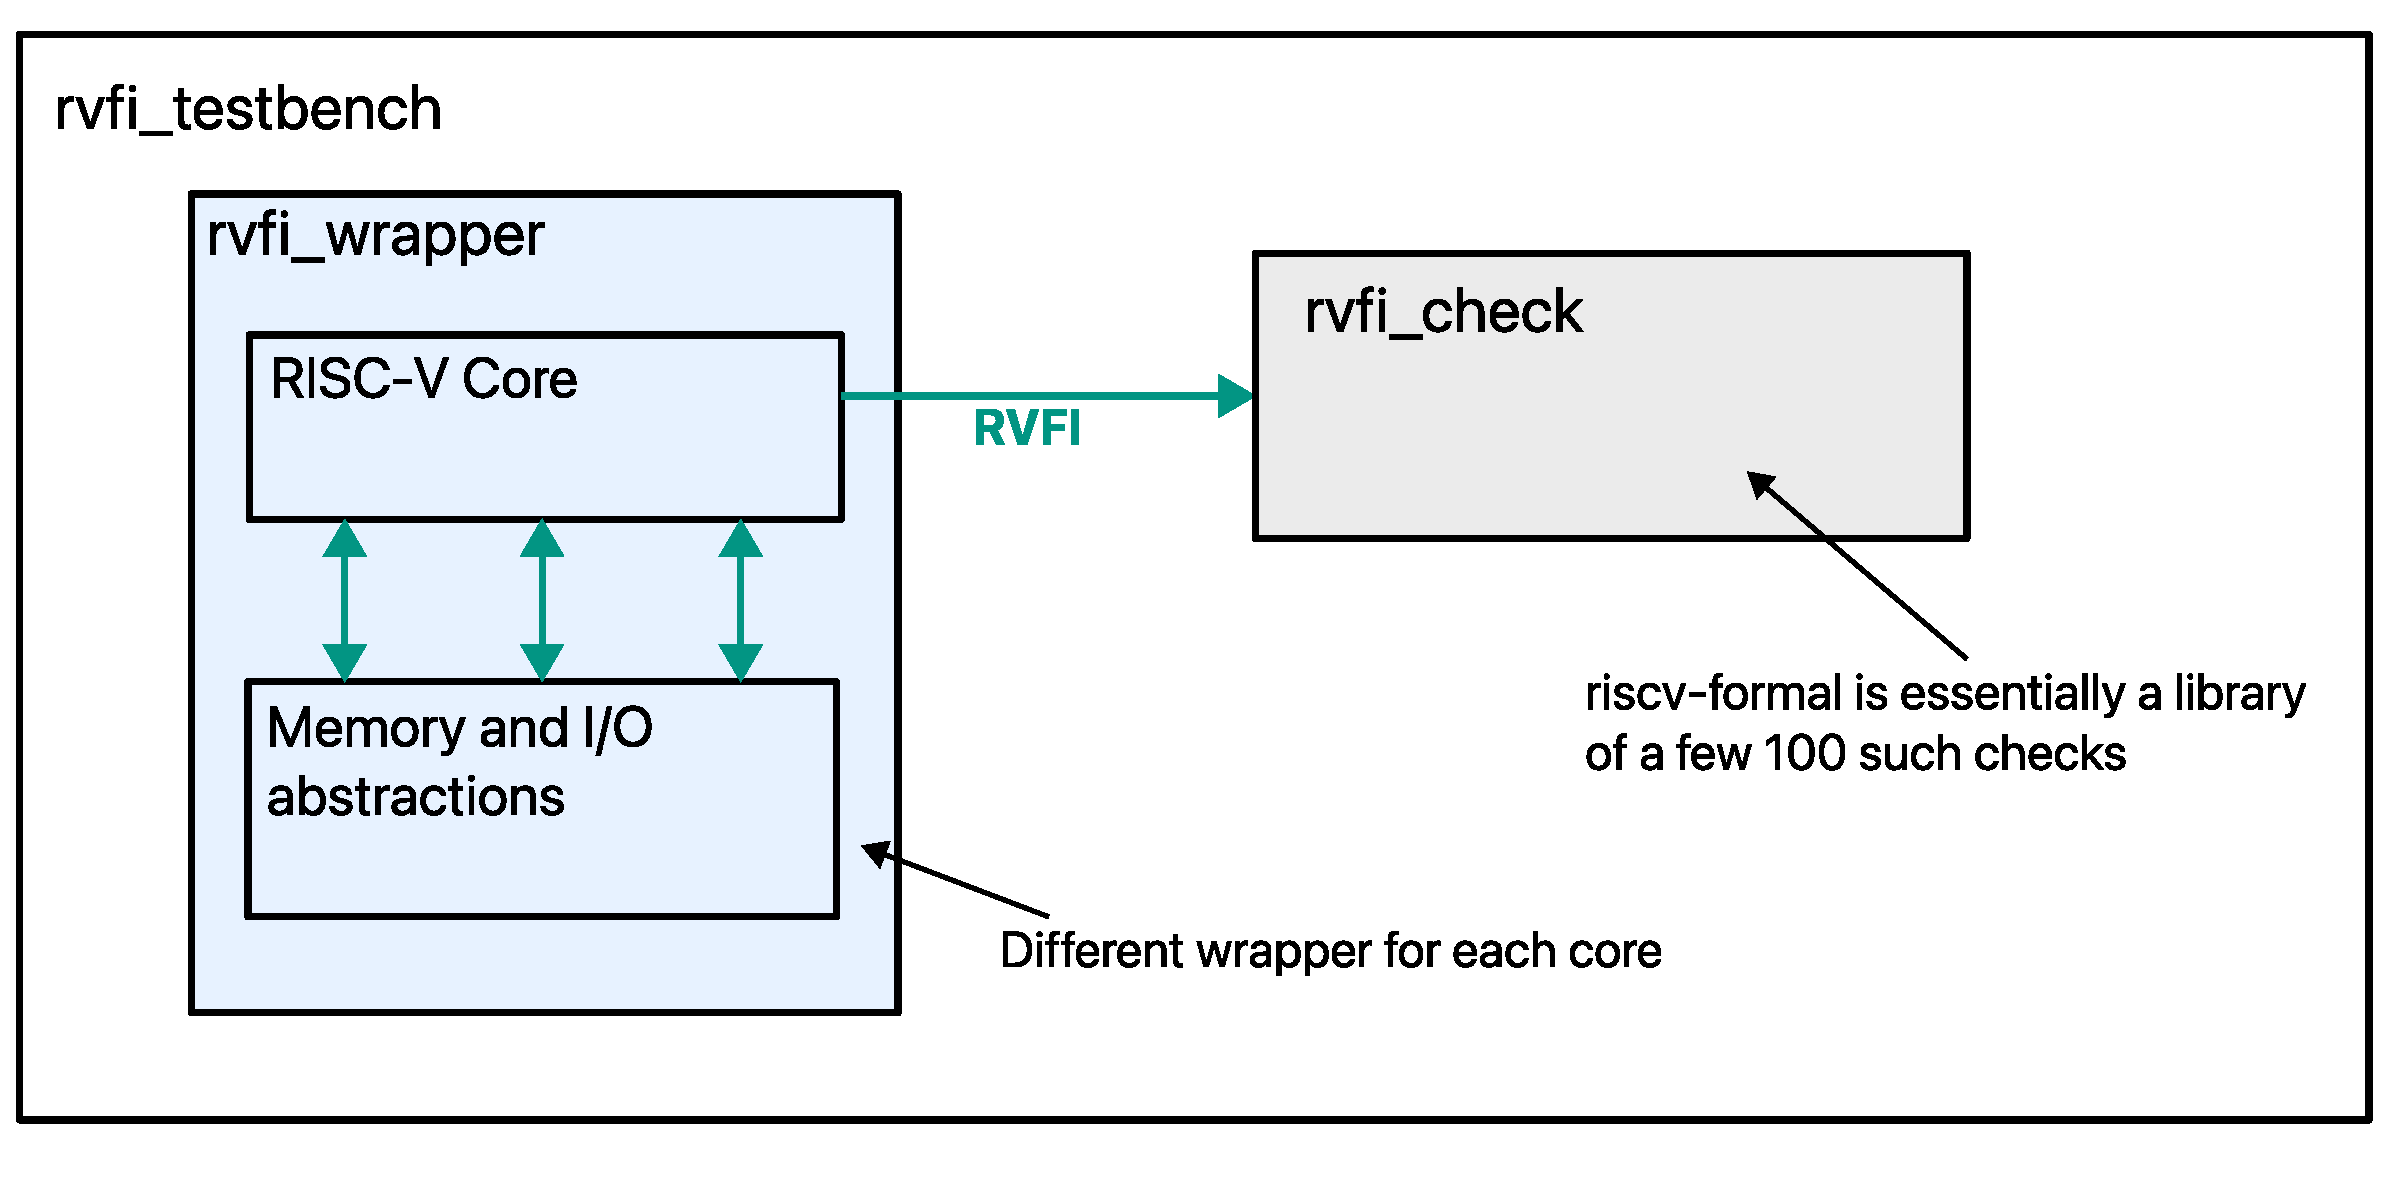
\includegraphics[width=1\linewidth]{pics/riscvformal.pdf}
    \caption{RISC-V Formal Framework Design}
    \label{fig: riscvformal}
    \end{center}
\end{figure}
% 图 1 是 RISC-V Formal 的框架设计。
Figure 1 shows the framework design of the RISC-V Formal.
% 首先,在对处理器正确性对验证过程中,内存和外部的 IO 会被抽象掉,连接核心的实现。
First of all, in the process of verifying the correctness of the processor, the memory and external IO will be abstracted and connected to the RISC-V core.
% 两者都作为 rvfi_wrapper 模块的组成。
Both are used as components of the \verb|rvfi_wrapper| module.
% 在核心中,需要实现 RVFI 接口,输出在指令执行过程中的一系列状态信息。
In the core, the RVFI interface needs to be implemented to output a series of state information during the instruction execution process.

\begin{lstlisting}[language=verilog, caption={RVFI Definition (partial)}, label=rvfi]
output [NRET        - 1 : 0] rvfi_valid,
output [NRET * ILEN - 1 : 0] rvfi_insn,
output [NRET *    5 - 1 : 0] rvfi_rs1_addr,
output [NRET * XLEN - 1 : 0] rvfi_rs1_rdata,
output [NRET * XLEN - 1 : 0] rvfi_pc_rdata,
output [NRET * XLEN - 1 : 0] rvfi_pc_wdata,
output [NRET * XLEN   - 1 : 0] rvfi_mem_addr,
output [NRET * XLEN   - 1 : 0] rvfi_mem_rdata,
output [NRET * XLEN   - 1 : 0] rvfi_mem_wdata
\end{lstlisting}

% 可以从上面的 Listing 1 中看到,RVFI 接口要求核心输出指令执行过程中指令编码的内容,指令的源操作数地址和内容,指令执行前后的 PC 值,以及内存访问的地址和内容等。
As shown in Listing \ref{rvfi}, the RVFI interface requires the core to output the contents of the instruction encoding, the source operand addresses and contents, the PC values before and after the instruction execution, and the addresses and contents of the memory access, etc.

% 之后,RVFI 接口作为 rvfi_check 模块的输入。
Then, the RVFI interface is used as the input of the \verb|rvfi_check| module.
% 在 RISC-V Formal 中,实际上包含了有几百个不同的 rvfi_check 模块。
There are actually a few hundred different \verb|rvfi_check| modules in RISC-V Formal.
% 这些多个小的 checker 模块分别对核心中不同方面的正确性进行验证。
These small checker modules verify the correctness of different aspects of the core separately.
% 例如有对 RISC-V 指令集中各个具体指令的执行正确性进行验证的 checkers,有对指令执行前后 PC 寄存器更新是否正确进行检查的 checker,有对通用寄存器值变化进行检查的,等等。
For example, there are checkers that verify the correctness of the execution of specific instructions in the RISC-V instruction set, checkers that check whether the PC register is updated correctly before and after the instruction execution, and checkers that check the change of the general register value, etc.
% 全部的检查内容可以查看项目文档或者相关代码。
All the check contents can be found in the project documentation or the related code \cite{riscv-formal}.

% 在一个具体的 checker 模块中,会包含一个实例化的对应的 spec 模块。在这个 spec 模块中,会依据 RISC-V 官方给出的规范内容来实现对应这一小块的规范内容。
Within a specific checker module, a corresponding spec module is instantiated. In this spec module, the corresponding small piece of specification is implemented according to the official RISC-V specification \cite{waterman2014risc}.
% 例如对于 |add| 指令验证的 checker 模块中,会实例化一个对应的 |insn_spec| 模块。在该模块中,会依据官方规范来定义对于加法指令,会对寄存器等状态变量产生怎样的影响。
For example, in the checker module of the \verb|add| instruction verification, a corresponding \verb|insn_spec| module is instantiated.
In this module, the impact on the registers and other state variables will be defined according to the official specification.
% |insn_spec| 模块会输出指令执行后各个状态变量的变化情况,然后在 checker 模块中,会使用 SVA 语法来描述 spec 输出结果和实际核心的执行情况是一致的断言。
The \verb|insn_spec| module outputs the changes in the state variables after the instruction execution, and then in the checker module, the SVA is used to describe the assertions that the spec output is consistent with the actual core execution.

% 最后,RISC-V Formal 会将这些包含 SVA 的 SystemVerilog 模块交给 SymbiYosys 工具来进行 BMC 检查。
Finally, RISC-V Formal hands over these SystemVerilog modules containing SVA to the SymbiYosys tool for BMC ( Bounded Model Checking) \cite{biere2009bounded}.
% 这里使用自动生成的 sby 文件来驱动 SymbiYosys。
Here, the automatically generated sby file is used to drive SymbiYosys.
% SymbiYosys 会给出性质验证的结果。由于只使用了 BMC 检查,因此只能给出在电路的若干步内,性质是否成立的结论。
SymbiYosys will give the results of the property verification. Since only BMC checking is used, only a conclusion can be given as to whether the property holds within a number of steps of the circuit.

% 基于 RISC-V Formal 的验证方法在业界得到了广泛的应用。
The RISC-V Formal-based verification approach is widely used in the industry. 
% Standard Semiconductor 的 Lion is a formally verified, 5-stage pipeline RISC-V core.
Standard Semiconductor's Lion is a formally verified, 5-stage pipeline RISC-V core.
% 它实现了 RVFI 接口并使用 RISC-V Formal 来进行形式化验证。
It implements the RVFI interface and uses RISC-V Formal for formal verification \cite{lion}.
% lowRISC 的 Ibex is a production-quality open source 32-bit RISC-V CPU core written in SystemVerilog. 它同样使用该框架进行形式化验证。
LowRISC's Ibex is a production-quality open source 32-bit RISC-V CPU core written in SystemVerilog. And it also uses this framework for formal verification \cite{ibex}.
WARP-V is a CPU generator written using Transaction-Level Verilog (TL-Verilog) that implements RISC-V ISA and has been formally verified using riscv-formal \cite{hoover2018formally}.

% 在 RISC-V Formal 中,由于底层使用 SVA 来定义性质,因此整个框架只适用于 SystemVerilog 实现的 RISC-V 处理器。
In RISC-V Formal, the entire framework is only applicable to SystemVerilog implementations of RISC-V processors because the underlying SVA is used to define the properties.
% 尽管,使用 Chisel 来设计和验证 RISC-V 处理器是更有生产力的,是大势所趋。
Although, using Chisel for designing and verifying RISC-V processors is more productive and is the general trend.
% 另一方面,RISC-V Formal 专注于进行 BMC,并且由于耦合强很难扩展到其他验证算法,或者是更换后端引擎。
On the other hand, RISC-V Formal is focused on BMC and is hard to extend to other verification algorithms or to replace the backend engine due to strong coupling.

\section{RISC-V Formal in Chisel}

% RVFC 是在 Chisel 层次对 RISC-V 处理器进行形式化验证的框架,其验证思路受启发于 RISC-V Formal 框架。
RVFC is a formal verification framework for RISC-V processors at the Chisel level, and its verification idea is inspired by the RISC-V Formal framework.
% 与 RISC-V Formal 不同,在 RVFC 中,对于形式化性质的定义和验证依赖于 ChiselFV。
Unlike RISC-V Formal, in RVFC, the definition and verification of formal properties depend on ChiselFV.
% ChiselFV 采用与 Chisel 相同的高级语言 Scala 语言实现,借助现代软件编程语言的高级特性,ChiselFV 具有很强的模块化和可扩展性。
ChiselFV is implemented in the Scala language, which is the same as Chisel. With the help of the advanced features of modern software programming languages, ChiselFV has strong modularity and extensibility.
% ChiselFV 目前支持直接调用 BMC, K-Induction, PDR 三种主流模型检测算法,同时其后端引擎易于插拔更换。
ChiselFV currently supports direct invocation of three mainstream model detection algorithms, BMC, K-Induction, and PDR. At the same time, its backend engine is easy to plug and replace.

% 本章节将通过两部分来详细说明 RVFC 框架,分别是 RVFC 的框架结构和验证流程。
This section details the RVFC framework in two parts, the framework structure and the verification workflow.

\subsection{Framework Structure}
% RVFC 的框架结构与 RISC-V Formal 类似,都需要 chip 实现 RVFI 接口,并将指令执行过程中的相关信息进行输出,最终与按照规范会达到的结果进行一致性断言。
The RVFC framework structure is similar to RISC-V Formal in that it requires the chip to implement the RVFI interface and output information about the instruction execution process, and finally assert consistency with the results that would be achieved according to the specification.

\begin{figure}[!htbp]
    \begin{center}
    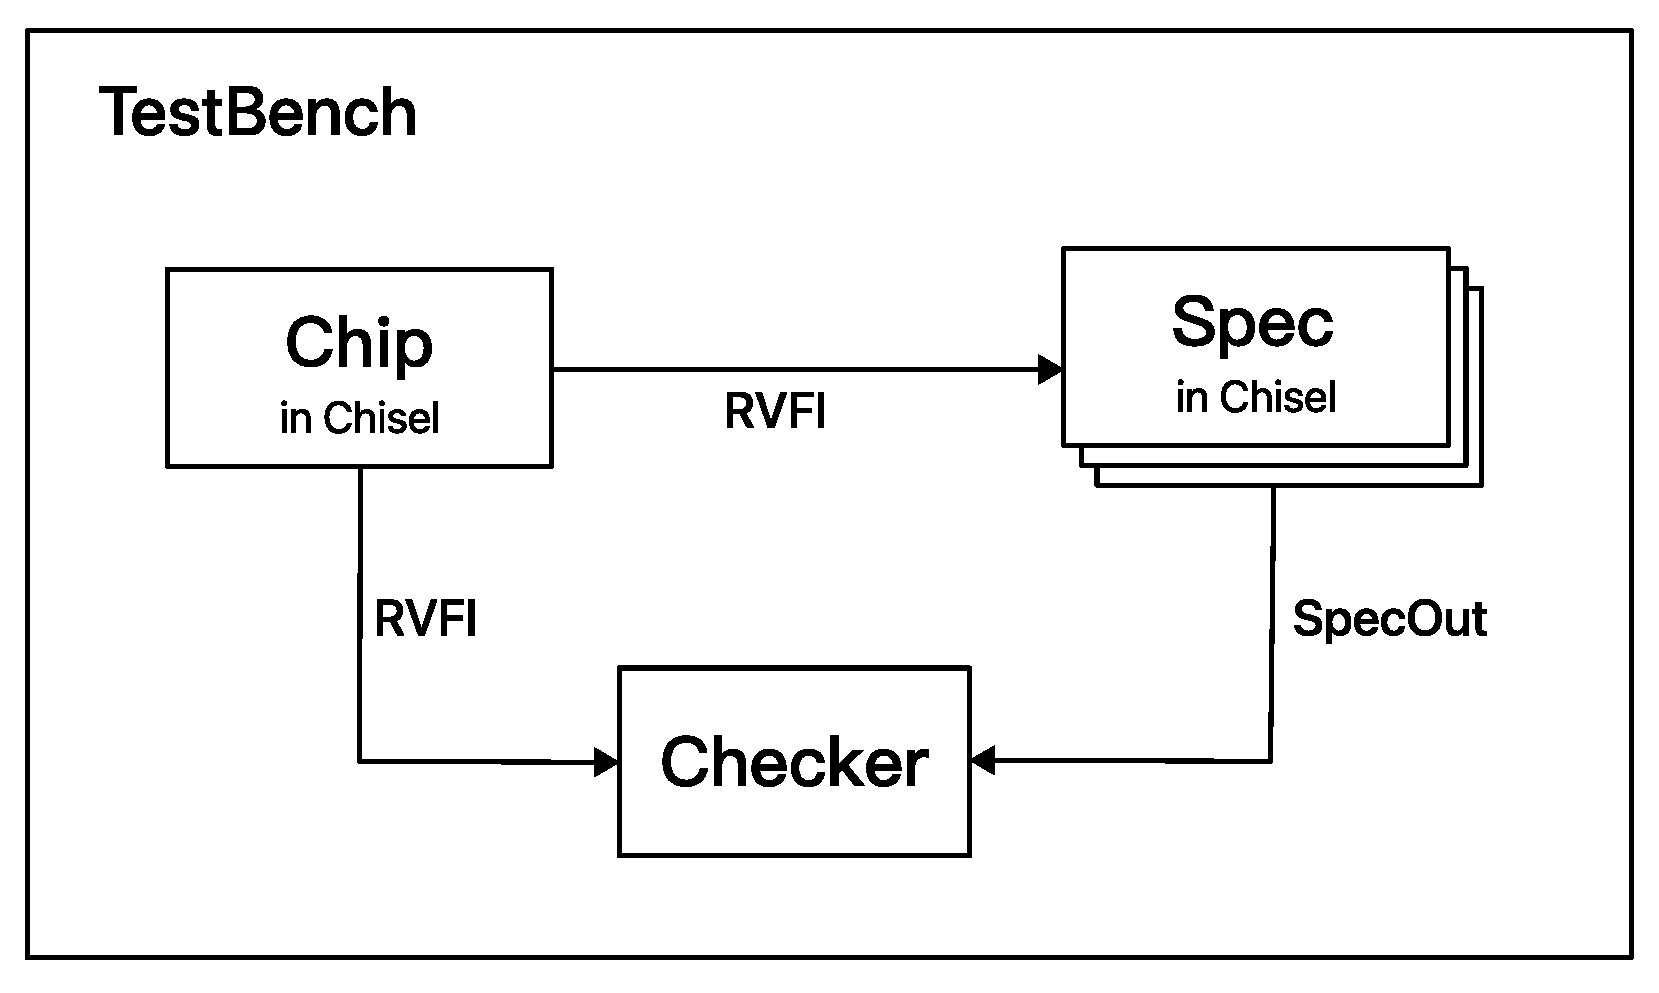
\includegraphics[width=1\linewidth]{pics/rvfc.pdf}
    \caption{RVFC Framework Structure}
    \label{fig: rvfc structure}
    \end{center}
\end{figure}

% 如图 2 所示,RVFC 验证框架中主要有三个主体,分别为: 使用 Chisel 实现的 RISC-V 处理器 Chip 模块即验证的对象,制定具体验证内容的 Spec 模块们和驱动验证过程的 Checker 模块。
As shown in Figure \ref{fig: rvfc structure}, there are three main bodies in the RVFC framework, namely: the RISC-V processor Chip module implemented by Chisel, which is the verification object, the Spec modules, which specify the verification content, and the Checker modules that drive the verification process.

\begin{lstlisting}[language=scala, caption={RVFI Definition in RVFC}, label=rvfic]
class RVFI_IO extends Bundle {
    val valid     = Output(Bool())
    val insn      = Output(UInt(32.W))
    val pc_rdata  = Output(UInt(64.W))
    val pc_wdata  = Output(UInt(64.W))
    val rs1_addr  = Output(UInt(5.W))
    val rs2_addr  = Output(UInt(5.W))
    val rs1_rdata = Output(UInt(64.W))
    val rs2_rdata = Output(UInt(64.W))
    val rd_addr   = Output(UInt(5.W))
    val rd_wdata  = Output(UInt(64.W))
    val mem_addr  = Output(UInt(32.W))
    val mem_rdata = Output(UInt(64.W))
    val mem_wdata = Output(UInt(64.W))
    val regs      = Vec(32, Output(UInt(64.W)))
}
\end{lstlisting}

% 与 RISC-V Formal 相同的,RVFC 中的 Chip 模块需要实现 RVFI 接口,将指令执行过程中的相关信息输出。
As in RISC-V Formal, the Chip module in RVFC needs to implement the RVFI interface and output information about the instruction execution process.
% 借助 Scala 语言更强的抽象能力,RVFI 接口被定义成一个 Bundle 的子类,从而更容易维护和扩展。
With the Scala language's greater abstraction capabilities, the \verb|RVFI_IO| is defined as a subclass of \verb|Bundle|, making it easier to maintain and extend.
% 比 RISC-V Formal 更多的是,RVFC 中将所有通用寄存器的状态作为 RVFI 的一部分进行输出,从而更好的检查指令执行的正确性。
In addition to RISC-V Formal, RVFC outputs the state of all general-purpose registers as part of RVFI, which is better for checking the correctness of instruction execution.

% |RVFI_IO| 作为 Chip 模块的输出,同时作为 Spec 模块们和 Checker 模块的输入。
The \verb|RVFI_IO| is the output of the Chip module and is also the input of the Spec modules and the Checker module.
% 同时在 RVFC 中,对于从 Chip 中引出的 RVFI 有时机上的要求。
In RVFC, there are also temporal requirements for RVFI from the Chip.
% 就是要求 RVFI 输出的时刻必须是在该指令提交前,而且在逻辑顺序上在该条指令之前的所有指令指令已经完成提交的之后。
That is, the RVFI output must be before the instruction is committed, and in the logical order, after all the instructions before the instruction have been committed.
% 换句话说,RVFI 需要输出逻辑上当前指令执行之前的状态信息,和该指令准备提交的信息。
In other words, RVFI needs to output the state information before the current instruction is executed, and the information that the instruction is ready to commit.
% 这也增加了该框架的可适用性,因为大多数流水线设计,即使是乱序执行,但是指令的提交仍然是按照指令原本的顺序的。
This also increases the applicability of the framework, because most pipeline designs, even if they are out-of-order, still commit instructions in the original order of the instructions.
% 如何在 Chip 中正确地进行 RVFI 的连接是整个验证工作中最困难的,这将在下一章节的研究案例中有所展示。
How to correctly connect RVFI in the Chip is the most difficult part of the verification work, which will be shown in the study case in the next section.

\begin{lstlisting}[language=scala, caption={SpecOut Definition in RVFC}, label=specout]
class SpecOut extends Bundle {
    val valid     = Output(Bool())
    val rs1_addr  = Output(UInt(5.W))
    val rs2_addr  = Output(UInt(5.W))
    val rs1_rdata = Output(UInt(64.W))
    val rs2_rdata = Output(UInt(64.W))
    val rd_addr   = Output(UInt(5.W))
    val rd_wdata  = Output(UInt(64.W))
    val pc_wdata  = Output(UInt(64.W))
    val mem_addr  = Output(UInt(32.W))
    val mem_wdata = Output(UInt(64.W))
}
\end{lstlisting}

% Spec 模块将 RVFI 作为输入,并输出 SpecOut。
The Spec module takes RVFI as input and outputs SpecOut.
% SpecOut 的定义如 Listing 3 所示。
The definition of \verb|SpecOut| is shown in Listing \ref{specout}.
% 其中的 |valid| 信号输出根据当前的 RVFI 输入,是否符合该验证项目的前提。
The \verb|valid| signal output is based on the current RVFI input, whether it meets the premise of the verification item.
% 例如,在对于指令 |add| 的功能性验证 Spec 模块中,只有当输入的指令格式为 |add|,而且流水线没有发生停滞或者中断时,该 |valid| 信号才会输出为 true。
For example, in the functional verification Spec module for the instruction \verb|add|, the \verb|valid| signal will only output \verb|true| when the instruction format is \verb|add| and the pipeline does not stall or interrupt.
% |SpecOut| 中其他的信号则是根据 RVFI 输入信息和需要验证的内容,使用组合电路,计算得到的规范下的正确的指令提交内容。
The other signals in \verb|SpecOut| are the correct instruction commit content under the specification, calculated by a combinational circuit based on the RVFI input information and the content to be verified.
% 例如对于 |add| 指令的验证,则是会输出根据指令解析得到的原操作数和目标操作数地址、按照地址从寄存器中取出的原操作数、计算得到的目标操作数等。
For example, for the \verb|add| instruction, the information about the source operands and target operands addresses, the source operands fetched from the registers according to the addresses, the target operands calculated and so on are output.

% 最后在 Checker 模块中,主要是对性质的定义和验证过程的驱动。
Finally, in the Checker module, it is mainly the definition of the properties and the driving of the verification process.
% 这里会对于 Chip 输出的 RVFI 和 Spec 模块们输出的 SpecOut 进行一致性的断言。
Consistency is asserted here between the RVFI output from Chip and the SpecOut output from the Spec modules.
% 在 Checker 模块中,可以对需要验证的性质内容,即对应的 Spec 模块们进行配置。
In the Checker module, the properties to be verified, that is, the corresponding Spec modules, can be configured.
% 用户可以增加或者减少此次需要验证的内容,也可以自定义编写 Spec 模块来进行验证。
Users can add or subtract content that needs to be validated this time, or write custom Spec modules to do so.
% 最后,用户可以配置选择调用 ChiselFV 的验证算法,目前提供了 BMC, K-induction, 和 PDR 算法。
Finally, users can configure the verification algorithm of ChiselFV to be called, and the BMC, K-induction, and PDR algorithms are currently provided.

\subsection{Verification Workflow}
% 使用 RVFC 对 Chisel 编写的 RISC-V 设计进行验证主要有以下几个步骤:首先需要在 Chip 这设计 RVFI 连接,接着配置需要验证的内容,最后配置需要调用的验证算法。
The verification of the RISC-V design in Chisel using RVFC consists of several steps: first, RVFI needs to be connected in Chip; then, the content to be verified needs to be configured; and finally, the verification algorithm to be called needs to be configured.
% RVFC 会调用 ChiselFV 的后端引擎进行验证,并给出验证结果,一般会有四种情况:性质成立、性质不成立、在当前算法下结果为未知、过长时间仍然没有结果。
RVFC calls the backend engine of ChiselFV for verification and gives the verification result, which is generally one of the following four cases: the property holds, the property does not hold, the result is unknown under the current algorithm, or the result is not obtained after a long time.

% 从 Chip 中引出 RVFI 信号是最有挑战性的一步,它要求编程人员对 Chip 的设计足够了解,或者是在进行 Chip 设计过程中就进行 RVFI 的连接。
The most challenging step is to extract the RVFI signal from Chip, which requires programmers to be sufficiently familiar with Chip design, or to connect RVFI during Chip design.
% 正如在前面中提到的,它要求是在每一条指令进行提交前,而且逻辑上在这条指令前的指令都已经完成提交的时刻,将机器状态信息、该条指令信息、该条指令准备提交的信息进行输出。
As mentioned earlier, it requires that the machine state information, the instruction information, and the information to be committed for this instruction be output at the time before this instruction is committed and after all the instructions that logically precede this instruction have been committed.
% 一方面这需要对 Chip 的设计足够了解。
On the one hand, this requires a sufficient understanding of Chip design.
% 另一方面,可能有些信息在流水线中因为冗余,在这一时刻已经被丢弃了。
On the other hand, some information may have been discarded in the pipeline due to redundancy at this time.
% 例如,在准备提交的时候,该条指令的原操作数可能已经无法获取了。
For example, the source operands of this instruction may no longer be available when it is ready to commit.
% 这在实践上需要对电路进行修改,或者是添加一些辅助电路来帮忙存储这些信息。
This requires modification of the circuit or the addition of some auxiliary circuits to help store this information in practice.

% 然后一步是对验证内容的配置。
The next step is the configuration of the verification content.
% RVFC 提供了一些基础的对于部分 RISC-V 指令的验证 Spec 模块们。
RVFC provides some basic Spec modules for the verification of some RISC-V instructions.
% 这些 Spec 模块们是根据 RISC-V 官方给出的指令集规范编写,定义了每条指令的正确行为。
These Spec modules are designed according to the RISC-V instruction set specification, and define the correct behavior of each instruction.
% 用户可以在实际运行的 Checker 模块中可选的配置这些 Spec 模块们。
Users can configure these Spec modules in the Checker module that runs in actual processing.
% 同时,用户也可以根据自己处理器正确性的具体需求,编写自己的 Spec 模块。
At the same time, users can also write their own Spec modules according to their specific requirements for processor correctness.
% 并加载到 Checker 模块中进行验证。
And load them into the Checker module for verification.

% 最后一步是对验证算法的配置。
The last step is the configuration of the verification algorithm.
% RVFC 是调用了 ChiselFV 的后端引擎进行验证的。ChiselFV 使用了 Scala 编写,模块化设计,后端引擎可以进行更改替换。
RVFC calls the backend engine of ChiselFV for verification. ChiselFV is written in Scala, modularly designed, and the backend engine can be changed and replaced.
% ChiselFV 默认提供的了调用 SymbiYosys 工具的验证引擎,提供了 BMC、K-Induction 和 PDR 算法。
By default, the ChiselFV provides a verification engine that calls the SymbiYosys, which provides BMC, K-Induction and PDR algorithms.
% BMC 算法的大概过程是直接将电路的状态转化为公式,在每一步使用求解器来判断是否出现不满足性质的解。
The approximate process of the BMC algorithm is to directly translate the state of the circuit into an equation and use a solver at each step to determine whether a solution appears that does not satisfy the property.
% 因此使用 BMC 算法只能得到在若干步内系统是否安全的结论,无法证明是否恒成立。
Therefore, the BMC algorithm can only obtain the conclusion that the system is safe within a certain number of steps, and cannot prove whether it is always true.
% 同时,随着步数的增加,求解公式的规模就会越大,求解时间会越来越长。
At the same time, as the number of steps increases, the size of the formula to be solved becomes larger and the solving time becomes longer.
% K-Induction 算法则是在 BMC 算法的过程中增加了一个检查,检查验证性质是否为 k 步归纳不变式。
The K-Induction algorithm, on the other hand, adds a check to the BMC algorithm process to check whether the property is a k-step inductive invariant.
% 因此 K-Induction 有可能会证明出性质恒成立,但是它的求解困难度也会随着步数增加而增加。
Therefore, K-Induction may prove that the property is always true, but the difficulty of solving it is also increasing with the increase of the number of steps.
% PDR 算法则是尝试通过维护一组公式序列,从而 without unrolling 的方式来进行求解,避免了每次求解公式的规模增加。
The PDR algorithm try to maintain a set of formula sequences to solve it without unrolling, thus avoiding the increase of the size of the formula to be solved each time.
% 但是随着步数增加,需要递归 block 的深度也会更大,求解时间也会越来越长。
However, as the number of steps increases, the depth of the recursive block also increases, and the solving time becomes longer \cite{vizel2015boolean}.
% 用户可以根据自己的需求选择不同的验证引擎。
Users can choose different verification engines according to their own needs.

\section{Case Study}
% 在本章节中,我们使用 Chisel 实现了经典架构教科书中介绍的一个五级流水线,并通过 RVFC 框架进行了形式化验证。
In this section, we use Chisel to implement a five-level pipeline introduced in a classic architecture textbook \cite{patterson2017computer} and formally verify it with the RVFC framework.
% 本章节分为三个部分:流水线设计、验证、结果与分析。
This section is divided into three parts: pipeline design, verification, and results and analysis.

\subsection{Pipeline Design}
% 在教科书 Computer Organization and Design RISC-V Edition 书中,为了直观说明指令集架构和处理器设计的内容,在第 4.13 节中一步步构建了一个五级流水线设计。
In the textbook \textit{Computer Organization and Design RISC-V Edition}, in order to intuitively explain the content of the instruction set architecture and processor design, a five-level pipeline design is built step by step in Section 4.13.
% 书中使用 Verilog 进行了实现,我们将书中给出的最后版本使用了 Chisel 语言进行了重新实现。
The book uses Verilog to implement it, and we re-implemented it using the Chisel language based on the final version given in the book.
% 处理器实现和验证的说明和代码也都在 RVFC 的仓库中,作为例子。
The description and code of processor implementation and verification are also in the repository of RVFC \cite{riscvFvChisel} as an example.

% 这是个简单的五级流水设计。
This is a simple five-level pipeline design. 
% 流水包括 指令取指、指令译码、指令执行、内存访问、写回。
The pipeline includes instruction fetch, instruction decode, instruction execution, memory access, and writeback.
% 指令执行上为单发射顺序执行。
Instruction execution is single-issue in-order execution.
% 它实现了 RISC-V 指令集四个典型的指令:|ld|, |sd|, |add| 和 |beq| 指令。
It implements four typical instructions of the RISC-V instruction set: \verb|ld|, \verb|sd|, \verb|add| and \verb|beq|.

% 在流水线设计中,采用了转发和停滞两种技术。
In the pipeline design, both forwarding and stalling techniques are used.
% 在指令在该流水线中执行的过程中,虽然指令的执行顺序是顺序的,但是相邻的指令会同时在执行过程中的不同阶段上。
During the execution of instructions in this pipeline, although the instructions are executed in sequential order, adjacent instructions can be executed at the same time but at different stages.
% 这样的流水设计会使得指令的执行更加高效,但是也引入了新的问题。
Such a pipeline design can make the execution of instructions more efficient, but it also introduces new problems.
% 这样的情境可能会发生:一条指令执行时依赖的寄存器数据正好是前面一条尚未提交的指令的写回数据。
Such a situation may occur: the register data that a certain instruction depends on is the writeback data of the previous instruction that has not yet been committed.
% 这就会导致 Data Hazards。
This leads to data hazards \cite{patterson2017computer}.
% 在该设计中,主要通过转发和停滞来解决这一问题。
In this design, the problem is mainly solved by forwarding and stalling.
% 转发是指,当被依赖的数据已经产生了,只是没有写回时,特判这种情况,并将在依赖该数据的地方直接将该数据作为输入。
Forwarding means that when the data being relied on has been generated and just not written back, this is specifically judged to be the case and the data is directly used as input at the place where the data is relied on.
% 当被依赖的数据还未产生或者计算出时,那么依赖的指令则需要停滞执行过程,并在流水中插入空指令 |nop|.
When the data being relied on has not yet been generated or calculated, the instruction that depends on it needs to stall the execution process and insert a \verb|nop| instruction in the pipeline.

% 关于流水想设计的详情,可以在项目仓库和教科书中找到。
For more details about pipeline design, you can find them in the project repository \cite{riscvFvChisel} and the textbook \cite{patterson2017computer}.

\subsection{Verification}
% 使用 RVFC 对 Chip 进行验证是通过前面提到的验证流程。
The verification of Chip is through the verification workflow mentioned above.
% 主要分为三步,分别是连接 RVFI 接口、配置验证内容和配置算法来驱动验证程序。
It mainly consists of three steps, namely connecting the RVFI interface, configuring the verification content, and configuring the algorithm to drive the verification process.

% 首先需要在处理器设计中实现 RVFI 接口。
First, the RVFI interface needs to be implemented in the processor design.
% 在指令准备提交的时候,关于该条指令的许多信息已经没有被存储了,例如源操作数地址、源操作数等。
At the time when the instruction is ready to be committed, many information about the instruction has been lost, such as the source operand address and source operand.
% 可以通过添加额外的寄存器存储这些信息。
These information can be stored by adding extra registers.
% 然而,ChiselFV 提供了 |past| 算子,用于获取某个电路节点在若干时刻前的状态。
However, ChiselFV provides the \verb|past| operator to get the status of a circuit node at some time in the past.
% 需要注意的是,如果使用该算子最远获取了之前 k 个时钟周期的某个信号的值,那么电路开始的前 k 个时钟周期内,|past| 算子拿不到数据。
Note that if the value of a signal in the previous k clock cycles is obtained by using the operator, the \verb|past| operator cannot get data in the first k clock cycles of the circuit.
% 在这个五级流水中,我们使用 |past| 算子最远获取了 3 个时钟之前的信息。
In this five-stage pipeline, the \verb|past| operator is used to fetch the information at the previous 3 clock cycles.
% 这里我们利用了 RVFI 接口中的 valid 信号来解决这个问题。
Here we use the \verb|valid| signal in the RVFI interface to solve this problem.
% 我们将电路第一次复位后的前三个时刻中 RVFI 中的 valid 信号置为 |false|.
We set the \verb|valid| signal in RVFI to \verb|false| in the first three clock cycles after the circuit is reset.
% 在连接 RVFI 信号连接时往往需要使用 |past| 算子来获取节点之前的信息。
When connecting the RVFI signal, it is often necessary to use the \verb|past| operator to obtain information about the node in the past.
% 这一步需要小心翼翼的完成,需要对流水线中电路十分的熟悉。
This step needs to be done carefully and requires a very good understanding of the circuit in the pipeline.
% 一方面为了指令执行的高效,往往会使得设计实现更加复杂,例如指令的源操作数可能是从寄存器文件中读取的,也可能是由转发机制得到。
On the one hand, in order to achieve high efficiency of instruction execution, the design implementation is often more complex, such as the source operand of the instruction may be read from the register file, or may be obtained by the forwarding mechanism.
% 另一方面,不同指令执行所需要的时间可能不同,例如对于直接从寄存器中取出数据并计算的指令可能比较快,然而对于一些需要访存的指令可能会需要更多的时钟周期。
On the other hand, the time required for different instructions to execute may be different, such as the instruction that directly takes the data from the register and calculates it may be faster, while the instruction that needs to access memory may require more clock cycles.
% 这些情况都会给 RVFI 接口的正确实现带来挑战。
These situations can bring challenges to the correct implementation of the RVFI interface.

% 下一步是对于验证内容的配置。
The next step is to configure the verification content.
% 在 RVFC 中,预设了一些 Spec 模块们,主要是对 RISC-V 指令集规范中的部分指令的规范进行了定义。
In RVFC, some Spec modules are preset, mainly to define some of the instructions in the RISC-V instruction set specification.
% 对于当前这个五级流水的例子,则只需要使用 |ld|, |sd|, |add| 和 |beq| 四条指令对应的 Spec 模块即可。
For the current example of a five-stage pipeline, only the Spec modules corresponding to the four instructions \verb|ld|, \verb|sd|, \verb|add| and \verb|beq| are needed.
% 我们将这些模块进行实例化后,将其输出连接到 Checker 模块中,即可完成配置。
We instantiate these modules and then connect their output to the Checker module to complete the configuration.
% 用户除了可以使用我们预设的 Spec 模块,也可以自己定义 Spec 模块。
In addition to using the Spec modules we preset, users can also define their own Spec modules.
% 这可以是对于扩展指令的行为定义,也可以是开发过程中一些类似于测试内容的性质描述。
This can be the definition of the behavior of the extended instruction, or the description of some properties similar to the test content in the development process.

% 最后一步是在 Checker 模块中配置验证算法。
The last step is to configure the verification algorithm in the Checker module.
% 在这个例子中,我们使用了 BMC 算法来检查前 20 步内所有的验证性质是否成立。
In this example, we use the BMC algorithm to check whether all the verification properties hold within the first 20 steps.
% 如 Listing 4 所示的为驱动验证过程的代码。
The code that drives the verification process is shown in Listing \ref{checkcode}.

\begin{lstlisting}[language=scala, caption={A Code Clip to Call Verification Process}, label=checkcode]
object testbench extends App {
    Check.bmc(() => new testbench, 20)
}
\end{lstlisting}

\subsection{Results and Analysis}

\section{Conclusion and Future Work}

\bibliographystyle{IEEEtran}
\bibliography{./ref.bib}

\end{document}
